\documentclass[11pt]{article}
\usepackage[margin=1in]{geometry}
\usepackage{amsmath,amssymb,booktabs,graphicx,hyperref}
\graphicspath{{../../docs/generated/planck_mes_first_paper/}}
\hypersetup{colorlinks=true,linkcolor=blue,citecolor=blue,urlcolor=blue}

\title{Finite-null calibration of MES-anchored low-multipole morphology in Planck PR3}
\author{Draft analysis note---nonauthoritative}
\date{26 August 2026}

\begin{document}
\maketitle

\begin{abstract}
The large-angle cosmic microwave background provides direct constraints on departures from an almost--Friedmann--Lema\^itre--Robertson--Walker geometry, but the Maartens--Ellis--Stoeger (MES) bounds are one-way, premise-dependent ceilings rather than measurements of shear, vorticity, or geometric family. We apply typed geodesic squared normalized MES ceiling coordinates to corrected Planck PR3 SMICA low-multipole features and calibrate them with the same frozen operator on 300 ordered paired FFP10 CMB+noise realizations. The analysis combines two realization-conditional squared normalized MES ceiling coordinates with eight dimensionless irreducible morphology coordinates and uses observation-inclusive leave-one-out finite ranks. The MES-family rank is $\frac{98}{301}\simeq 0.326$, compared with $\frac{133}{301}\simeq 0.442$ for a separately frozen generic twelve-feature benchmark. The smallest coordinate rank is $\frac{16}{301}\simeq 0.053$ and comes from an octupole multipole-vector coordinate; the two MES ceilings each have rank $74/301\simeq 0.246$. The observation-row minimum is morphology-driven rather than anchor-driven. The full family rank nevertheless remains coordinate-family dependent, because adding the two MES ceilings changes the complete-pool row-score distribution. This is a conditional finite-null methods application, not a physical or geometric identification.
\end{abstract}

\section{Introduction and scope}
The MES programme derives comparatively model-independent one-way bounds on large-scale kinematic departures from CMB multipoles under stated almost-EGS assumptions \cite{MaartensEllisStoeger1995,StoegerAraujoGebbie1997}. A small CMB anisotropy can restrict admissible departures under those assumptions, but the converse does not follow: scalar ceilings do not select a geometry or provide posterior evidence for one.

Large-angle CMB studies also face a statistical family-selection problem. Correlated statistics are inspected on one observed sky, while apparent prominence can depend on cleaning, masks, and the chosen statistic family \cite{Planck2018VII,HeroldEtAl2025}. We therefore calibrate a predeclared family with an exact complete-pool rank, following the conservative nonzero finite-rank principle \cite{PhipsonSmyth2010}, rather than searching post hoc for a preferred anomaly statistic.

Our scope is narrow: construct typed same-row MES coordinates from corrected $C_2$ and $C_3$, combine them with eight frozen morphology coordinates, evaluate all six predeclared family variants, and state the remaining nonidentification boundaries. This draft neither reopens maps nor extends the ensemble after seeing the result.

\section{Planck PR3 observation and paired FFP10 null ensemble}
The observation is Planck PR3 SMICA temperature data represented by the committed joint cut-sky low-$\ell$ feature row; SMICA and the PR3 component products are described by Planck Collaboration IV \cite{Planck2018IV}. The null pool contains 300 exact ordered pairs of FFP10 SMICA CMB and noise realizations. Every row has the same mask, harmonic convention, beam/pixel commonization, feature order, and numerical operator. The portable generic row is
\[
(C_2,C_3,C_4,C_5,\mathcal P,G_2,G_3,d_2,d_{3,0},d_{3,1},d_{3,2},A_{23}).
\]
The primary scope is conditional on this one SMICA row and this fixed pool. Other component-separation products and larger robustness ensembles are outside the present analysis.

\section{Corrected joint cut-sky low-ell features}
The corrected estimator fits all real harmonics through $\ell=5$ simultaneously on the weighted cut sky. Monopole and dipole coefficients are nuisance terms in the same fit as the retained $\ell=2,\ldots,5$ modes; only after the masked fit are retained coefficients mapped to the common beam/pixel convention. The registered basis and retained dimensions are 36 and 32, respectively. The condition number is 6.207504, and the relative singular floor is 0.159989. The corrected generic family reproduces the frozen $\frac{133}{301}$ benchmark rank.

\section{Typed squared normalized MES realization-conditional ceilings}
For each row,
\[
\epsilon_\ell=\frac{1}{T_0}\left[\frac{(2\ell+1)C_\ell}{4\pi}\right]^{1/2}.
\]
Under the registered SAG observer-motion branch, the residual cosmological dipole attribution is $\epsilon_1=0$. Define the squared normalized targets
\[
\Sigma^2\equiv\frac{\sigma_{ab}\sigma^{ab}}{6H^2},
\qquad
W^2\equiv\frac{\omega_{ab}\omega^{ab}}{6H^2}.
\]
The active geodesic MES factory supplies the one-way ceilings
\[
\Sigma^2\leq\Sigma^2_{\max}=\frac32\left(3\epsilon_2+\frac37\epsilon_3\right)^2,
\qquad
W^2\leq W^2_{\max}=\frac32\left(\frac{2}{15}\epsilon_2\right)^2.
\]
These squared normalized MES ceiling coordinates are deterministic functions of each row's $C_2$ and $C_3$, share the same data, and are not observed physical shear or vorticity. The MES family is
\[
(\Sigma^2_{\max},W^2_{\max},\mathcal P,G_2,G_3,d_2,d_{3,0},d_{3,1},d_{3,2},A_{23}).
\]

\begin{table}[ht]
\centering
\small
\caption{Premises and normalization of the registered MES ceiling coordinates. These assumptions are part of the interpretation, not conclusions inferred from the data.}
\begin{tabular}{p{0.24\linewidth}p{0.66\linewidth}}
\toprule
Item & Registered premise \\
\midrule
Congruence & geodesic \\
Regime & linear almost-EGS \\
Dipole attribution & SAG observer-motion; residual $\epsilon_1=0$ \\
Conditioning & realization-conditional same-row \\
Shear normalization & $\sigma_{ab}\sigma^{ab}/(6H^2)$ \\
Vorticity normalization & $\omega_{ab}\omega^{ab}/(6H^2)$ \\
$C_1/C_2$ status & premise-dependent derivative hierarchy \\
Converse & forbidden; a ceiling coordinate is not a measured invariant \\
\bottomrule
\end{tabular}
\label{tab:mes-premises}
\end{table}

\section{Observation-inclusive finite-null family statistic}
Let $X_{ij}$ be coordinate $j$ of row $i$ in the complete $N=301$ pool. For every two-sided coordinate, $m_{ij}$ is the median after excluding row $i$, and $D_{ij}=|X_{ij}-m_{ij}|$. The local complete-pool rank is
\[
p_{ij}=\frac1N\sum_{k=1}^N\mathbf 1(D_{kj}\ge D_{ij}).
\]
With $r_i=\min_j p_{ij}$, the family rank for the observation is
\[
p_{\rm fam}=\frac1N\sum_{i=1}^N\mathbf 1(r_i\le r_{\rm obs}).
\]
This operator is equivariant under complete-row permutations, includes the selected row, and treats ties conservatively.

\paragraph{Calibration premise.}
Under the null premise that the observed SMICA row and the 300 processed FFP10 rows are jointly exchangeable under the null, the complete row-scoring map is permutation-equivariant. Hence the observation-inclusive family rank is super-uniform, with conservative treatment of ties \cite{PhipsonSmyth2010,BarberRamdas2026}. If FFP10 does not faithfully represent the observational null, the reported fractions remain exact empirical ranks relative to the frozen pool, but they do not inherit unconditional Type-I-error calibration. Arithmetic exactness of the finite-pool rank is therefore distinct from scientific fidelity of the null model.

\section{Results}
\subsection{Coordinate-wise ranks}
\begin{table}[ht]
\centering
\caption{MES-family observed coordinates and finite ranks. The table is diagnostic-only (C2); it does not assign physical sources.}
\begin{tabular}{lrr}
\toprule
Coordinate & Observed value & Finite rank \\
\midrule
$\Sigma^2_{\max}$ & $2.4000870e-10$ & $\frac{74}{301}$ \\
$W^2_{\max}$ & $3.0061888e-13$ & $\frac{74}{301}$ \\
parity & $0.553365$ & $\frac{95}{301}$ \\
$G_2$ & $0.449993$ & $\frac{182}{301}$ \\
$G_3$ & $0.560137$ & $\frac{35}{301}$ \\
$d_2$ & $0.133173$ & $\frac{177}{301}$ \\
$d_{3,0}$ & $0.398744$ & $\frac{16}{301}$ \\
$d_{3,1}$ & $0.433858$ & $\frac{155}{301}$ \\
$d_{3,2}$ & $0.436828$ & $\frac{174}{301}$ \\
$A_{23}$ & $0.940239$ & $\frac{135}{301}$ \\
\bottomrule
\end{tabular}
\label{tab:coordinate-ranks}
\end{table}

The two squared normalized MES ceilings each have rank $74/301$, whereas the smallest coordinate rank is $\frac{16}{301}$ from $d_{3,0}$. The same $d_{3,0}$ minimum and rank occur in the morphology-only family. Thus the observation-row minimum is morphology-driven rather than anchor-driven. This statement concerns the minimum coordinate only, not the complete-pool family-rank distribution.

\begin{figure}[ht]
\centering
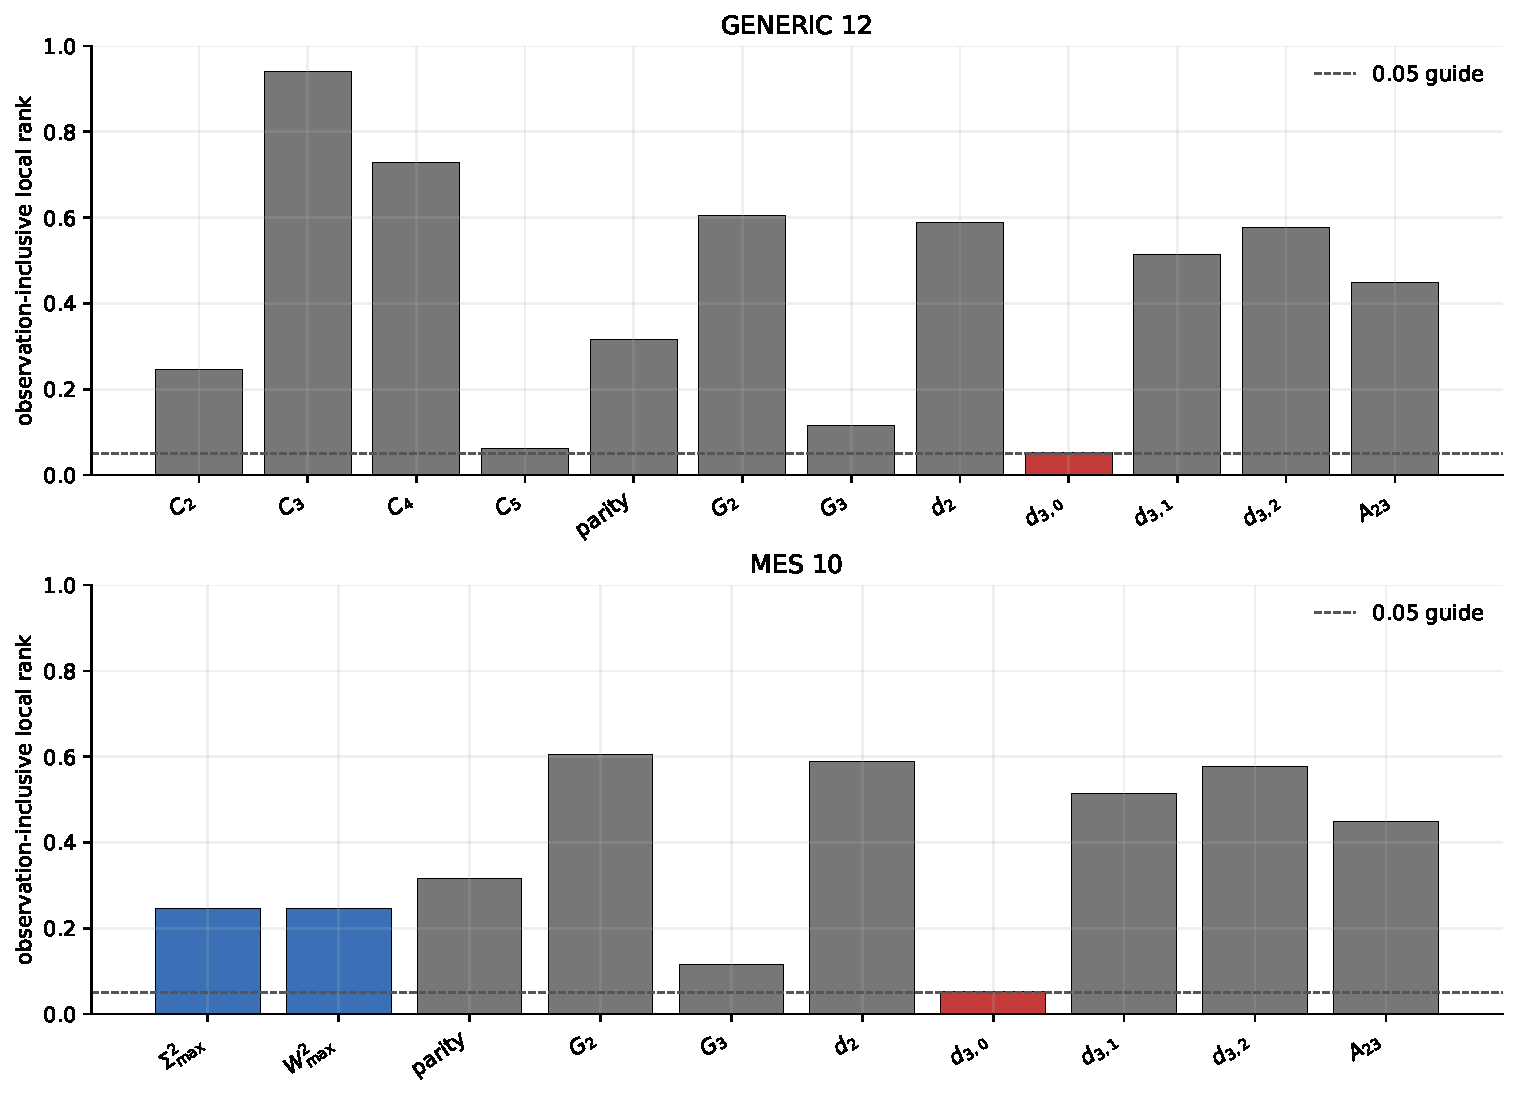
\includegraphics[width=0.96\linewidth]{figure_local_rank_profile.pdf}
\caption{Observation-inclusive local ranks for the generic and MES families. Red marks the family minimum; blue marks the squared normalized MES ceiling coordinates. This C2 diagnostic shows coordinate ranks only and supplies no directional or geometric identification.}
\label{fig:local-ranks}
\end{figure}

\subsection{Family decomposition and coordinate sensitivity}
\begin{table}[ht]
\centering
\small
\caption{Six predeclared family variants on the identical 301-row pool. Rank differences are descriptive paired operator sensitivity, not separate tests.}
\begin{tabular}{p{0.18\linewidth}p{0.38\linewidth}rr}
\toprule
Family & Purpose & Global rank & Minimum coordinate \\
\midrule
GENERIC\_12 & frozen generic twelve-feature benchmark control & $\frac{133}{301}$ & $d_{3,0}$ ($\frac{16}{301}$) \\
RAW\_REDUCED\_10 & isolates removal of raw C4 and C5 & $\frac{110}{301}$ & $d_{3,0}$ ($\frac{16}{301}$) \\
EPS\_REDUCED\_10 & isolates the C\_l-to-dimensionless-amplitude transformation & $\frac{109}{301}$ & $d_{3,0}$ ($\frac{16}{301}$) \\
MES\_10 & primary typed squared MES-ceiling plus morphology family & $\frac{98}{301}$ & $d_{3,0}$ ($\frac{16}{301}$) \\
ANCHORS\_ONLY\_2 & measures anchor-only extremeness and dependence & $\frac{78}{301}$ & $\Sigma^2_{\max}$, $W^2_{\max}$ ($\frac{74}{301}$) \\
MORPHOLOGY\_ONLY\_8 & isolates the irreducible morphology contribution & $\frac{88}{301}$ & $d_{3,0}$ ($\frac{16}{301}$) \\
\bottomrule
\end{tabular}
\label{tab:family-decomposition}
\end{table}

Removing $C_4$ and $C_5$ changes the global rank from $\frac{133}{301}$ to $\frac{110}{301}$. Replacing $(C_2,C_3)$ by $(\epsilon_2,\epsilon_3)$ gives $\frac{109}{301}$, and replacing those amplitudes by the two registered squared normalized MES ceiling coordinates gives $\frac{98}{301}$. The ceilings-only and morphology-only ranks are $\frac{78}{301}$ and $\frac{88}{301}$. No difference between these fractions is assigned a separate significance.

Across all 301 rows the anchor Pearson correlation is 0.994874, and the Spearman correlation is 0.993738. The two-by-two correlation block has numerical rank 2 and condition number 389.165. These values quantify strong shared same-row dependence; they do not establish additional information.

\begin{table}[ht]
\centering
\scriptsize
\caption{Spearman dependence of complete-row family scores. These paired descriptive values are not a multiple-testing panel.}
\begin{tabular}{llr}
\toprule
Family A & Family B & Spearman $\rho$ \\
\midrule
GENERIC\_12 & RAW\_REDUCED\_10 & 0.8608 \\
GENERIC\_12 & EPS\_REDUCED\_10 & 0.8413 \\
GENERIC\_12 & MES\_10 & 0.7684 \\
GENERIC\_12 & ANCHORS\_ONLY\_2 & 0.1335 \\
GENERIC\_12 & MORPHOLOGY\_ONLY\_8 & 0.7305 \\
RAW\_REDUCED\_10 & EPS\_REDUCED\_10 & 0.9834 \\
RAW\_REDUCED\_10 & MES\_10 & 0.8933 \\
RAW\_REDUCED\_10 & ANCHORS\_ONLY\_2 & 0.1455 \\
RAW\_REDUCED\_10 & MORPHOLOGY\_ONLY\_8 & 0.8472 \\
EPS\_REDUCED\_10 & MES\_10 & 0.8959 \\
EPS\_REDUCED\_10 & ANCHORS\_ONLY\_2 & 0.1470 \\
EPS\_REDUCED\_10 & MORPHOLOGY\_ONLY\_8 & 0.8606 \\
MES\_10 & ANCHORS\_ONLY\_2 & 0.1893 \\
MES\_10 & MORPHOLOGY\_ONLY\_8 & 0.9457 \\
ANCHORS\_ONLY\_2 & MORPHOLOGY\_ONLY\_8 & 0.0429 \\
\bottomrule
\end{tabular}
\label{tab:score-dependence}
\end{table}

\begin{figure}[ht]
\centering
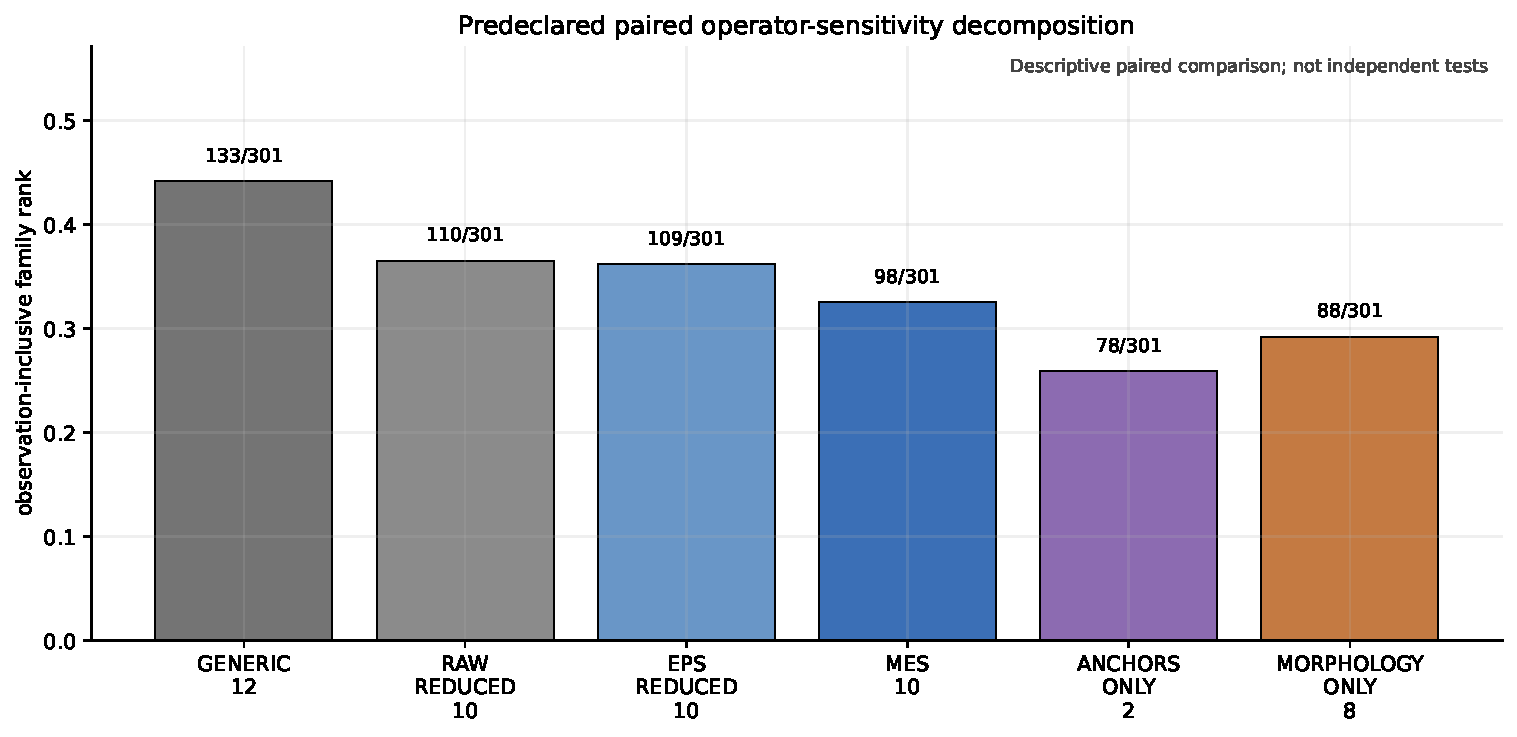
\includegraphics[width=0.96\linewidth]{figure_family_rank_comparison.pdf}
\caption{Six-family observation-inclusive rank comparison. This C2 diagnostic separates coordinate/family choices; it does not measure a physical effect of MES reparameterization.}
\label{fig:family-ranks}
\end{figure}

\begin{figure}[ht]
\centering
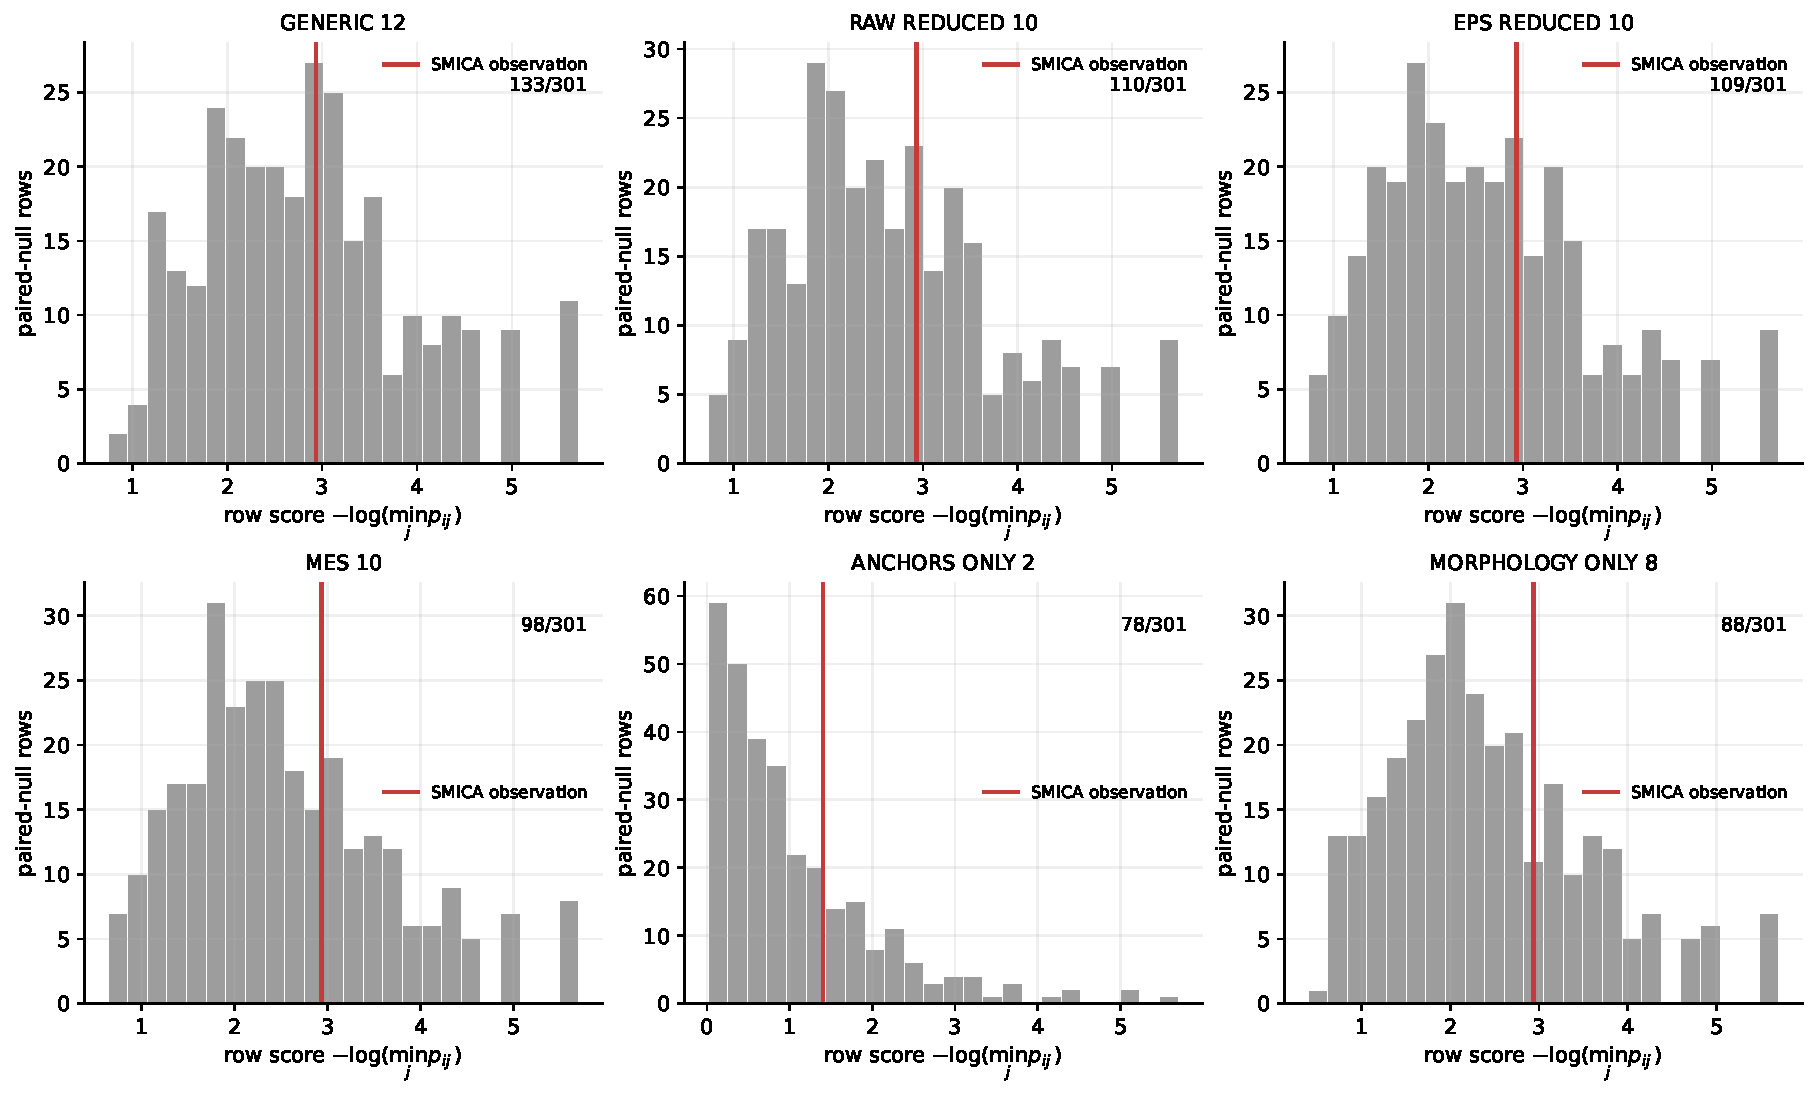
\includegraphics[width=0.98\linewidth]{figure_global_null_scores.pdf}
\caption{Complete-pool row-score distributions with the SMICA observation marked. The covariance exported by PR-327 is not used in these ranks or histograms.}
\label{fig:global-scores}
\end{figure}

\begin{figure}[ht]
\centering
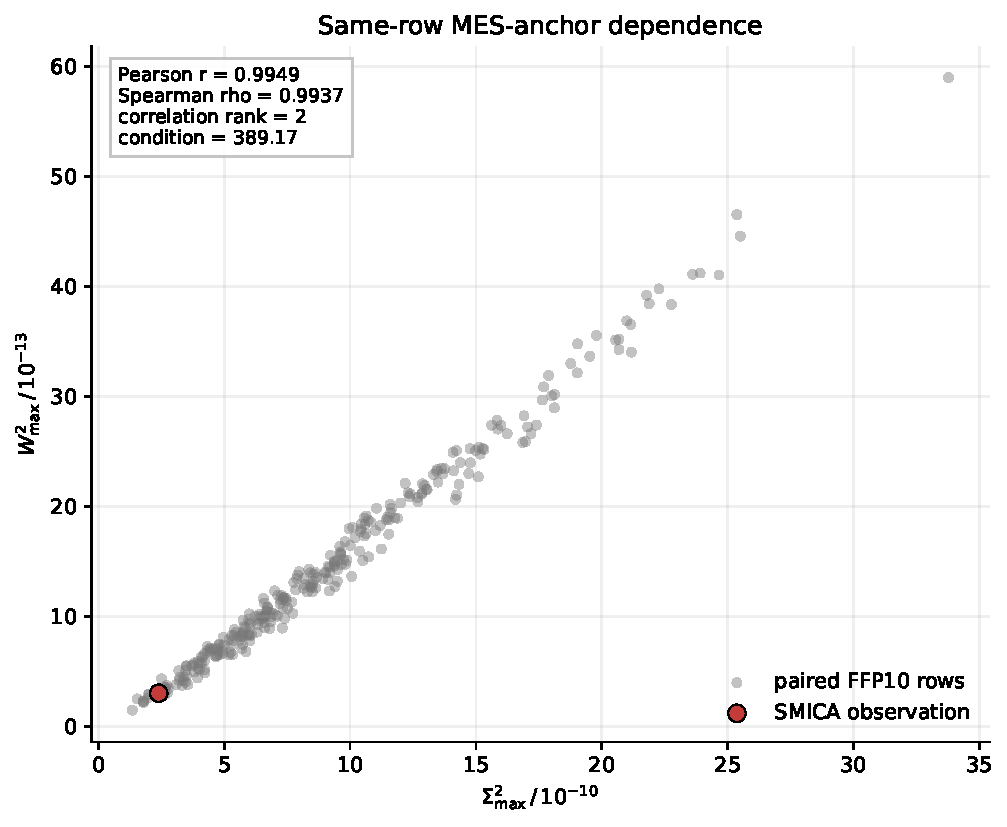
\includegraphics[width=0.72\linewidth]{figure_anchor_dependence.pdf}
\caption{Dependence of the two realization-conditional squared normalized MES ceilings across the fixed pool. Their strong association is expected from shared $C_2,C_3$ inputs and does not imply two independent channels.}
\label{fig:anchor-dependence}
\end{figure}

\subsection{Generic-control comparison}
The MES-family rank $\frac{98}{301}$ and generic-control rank $\frac{133}{301}$ are outputs of two different predeclared coordinate families on the same rows. The decomposition in Table~\ref{tab:family-decomposition} shows that the change combines removal of two raw amplitudes with two coordinate transformations. It is therefore inappropriate to attribute the full numerical change to MES physics.

\section{Interpretation and limitations}
The primary result is a null result within the frozen finite ensemble: the family rank is not unusually small, and the observation-row minimum coordinate is an octupole morphology statistic rather than either MES ceiling. The full family rank nevertheless remains coordinate-family dependent, because adding the two MES ceilings changes the complete-pool row-score distribution. This supports the operational use and map-free calibration of typed MES ceiling coordinates, while supplying no measurement of physical shear or vorticity.

The main limitations are one SMICA component-separation product, 300 paired CMB+noise rows, realization-conditional same-row anchors, no direction-indexed source field in the portable package, no physical response that separates local and global contributions, and no native-solver morphology atlas. Planck-only local/global separation is nonidentified, and scalar coordinates cannot construct a direction or STF object. The pooled ten-dimensional covariance is a conditioning diagnostic only; it is absent from the rank scan and from any likelihood.

\section{Conclusion}
We constructed a typed, row-equivariant finite-null application of geodesic squared normalized MES ceiling coordinates to Planck PR3 low-multipole morphology. Within the frozen SMICA plus 300 paired FFP10 ensemble, the ten-coordinate family rank is $\frac{98}{301}$. Its observation-row minimum is $\frac{16}{301}$ and is morphology-driven rather than anchor-driven. The family rank remains coordinate-family dependent: the morphology-only rank is $\frac{88}{301}$, while adding the two ceilings changes the complete-pool row-score distribution and gives $\frac{98}{301}$. The analysis is a reproducible methodological bridge and conditional null result. It does not identify a physical source, distinguish local from global kinematics, or select a Bianchi geometry.

\appendix
\section{Exact morphology definitions and conventions}
The eight morphology coordinates use the same frozen operator on every row. The even-to-odd low-multipole power ratio is
\[
\mathcal P=\frac{C_2+C_4}{C_3+C_5}.
\]
For each $\ell\in\{2,3\}$, let $A^{(\ell)}$ be the real symmetric trace-one angular-momentum power tensor, with ordered eigenvalues $\lambda_{\ell,1}\leq\lambda_{\ell,2}\leq\lambda_{\ell,3}$. The registered power-tensor gap is
\[
G_\ell=\lambda_{\ell,3}-\lambda_{\ell,2}.
\]
This construction follows the angular-momentum power-tensor family of directional statistics \cite{AluriRalstonWeltman2017}.

Multipole vectors are extracted from the Majorana polynomial
\[
P_\ell(z)=\sum_{m=-\ell}^\ell
\sqrt{\binom{2\ell}{\ell+m}}\,a_{\ell m}z^{\ell+m},
\]
using orthonormal Condon--Shortley harmonics and $z=e^{i\phi}\cot(\theta/2)$. Antipodally paired roots define unoriented axes $\boldsymbol v_{\ell,i}$; the stored representative has its largest-absolute Cartesian component positive \cite{CopiHutererStarkman2004,Weeks2004}. The quadrupole coordinate is
\[
d_2=\left|\boldsymbol v_{2,1}\!\cdot\!\boldsymbol v_{2,2}\right|.
\]
For the octupole, the three absolute pairwise products are sorted in ascending order:
\[
(d_{3,0},d_{3,1},d_{3,2})
=\operatorname{sort}\left\{
\left|\boldsymbol v_{3,i}\!\cdot\!\boldsymbol v_{3,j}\right|:
1\leq i<j\leq3
\right\}.
\]
Finally, define the normalized quadrupole plane normal $\widehat{\boldsymbol n}_2$ from $\boldsymbol v_{2,1}\times\boldsymbol v_{2,2}$ and the three normalized octupole plane normals $\widehat{\boldsymbol n}_{3,ij}$ from $\boldsymbol v_{3,i}\times\boldsymbol v_{3,j}$. The plane-alignment coordinate is
\[
A_{23}=\max_{i<j}
\left|\widehat{\boldsymbol n}_2\!\cdot\!\widehat{\boldsymbol n}_{3,ij}\right|.
\]
Degenerate coincident axes make the corresponding plane undefined and are rejected by the frozen operator rather than assigned an artificial direction.

\section{Exact feature and tail registry}
Every listed coordinate uses a two-sided tail and the same observation-inclusive scan.
\begin{description}
\item[GENERIC\_12] \texttt{cl\_l2}, \texttt{cl\_l3}, \texttt{cl\_l4}, \texttt{cl\_l5}, \texttt{parity\_even\_over\_odd\_l2\_l5}, \texttt{power\_tensor\_gap\_l2}, \texttt{power\_tensor\_gap\_l3}, \texttt{multipole\_l2\_absdot}, \texttt{multipole\_l3\_absdot\_0}, \texttt{multipole\_l3\_absdot\_1}, \texttt{multipole\_l3\_absdot\_2}, \texttt{multipole\_plane\_alignment\_max\_l2\_l3}
\item[RAW\_REDUCED\_10] \texttt{cl\_l2}, \texttt{cl\_l3}, \texttt{parity\_even\_over\_odd\_l2\_l5}, \texttt{power\_tensor\_gap\_l2}, \texttt{power\_tensor\_gap\_l3}, \texttt{multipole\_l2\_absdot}, \texttt{multipole\_l3\_absdot\_0}, \texttt{multipole\_l3\_absdot\_1}, \texttt{multipole\_l3\_absdot\_2}, \texttt{multipole\_plane\_alignment\_max\_l2\_l3}
\item[EPS\_REDUCED\_10] \texttt{epsilon\_2}, \texttt{epsilon\_3}, \texttt{parity\_even\_over\_odd\_l2\_l5}, \texttt{power\_tensor\_gap\_l2}, \texttt{power\_tensor\_gap\_l3}, \texttt{multipole\_l2\_absdot}, \texttt{multipole\_l3\_absdot\_0}, \texttt{multipole\_l3\_absdot\_1}, \texttt{multipole\_l3\_absdot\_2}, \texttt{multipole\_plane\_alignment\_max\_l2\_l3}
\item[MES\_10] \texttt{mes\_sigma\_anchor}, \texttt{mes\_omega\_anchor}, \texttt{parity\_even\_over\_odd\_l2\_l5}, \texttt{power\_tensor\_gap\_l2}, \texttt{power\_tensor\_gap\_l3}, \texttt{multipole\_l2\_absdot}, \texttt{multipole\_l3\_absdot\_0}, \texttt{multipole\_l3\_absdot\_1}, \texttt{multipole\_l3\_absdot\_2}, \texttt{multipole\_plane\_alignment\_max\_l2\_l3}
\item[ANCHORS\_ONLY\_2] \texttt{mes\_sigma\_anchor}, \texttt{mes\_omega\_anchor}
\item[MORPHOLOGY\_ONLY\_8] \texttt{parity\_even\_over\_odd\_l2\_l5}, \texttt{power\_tensor\_gap\_l2}, \texttt{power\_tensor\_gap\_l3}, \texttt{multipole\_l2\_absdot}, \texttt{multipole\_l3\_absdot\_0}, \texttt{multipole\_l3\_absdot\_1}, \texttt{multipole\_l3\_absdot\_2}, \texttt{multipole\_plane\_alignment\_max\_l2\_l3}
\end{description}
The six families were fixed before their decomposition values were computed and are not interpreted as independent hypotheses.

\section{Map-free replay and data/code availability}
The paper builder reads the eight committed map-free inputs recorded in \path{docs/generated/planck_mes_first_paper/analysis_summary.json}. It generates three CSV tables, four diagnostic PDF figures, and this source draft without opening the raw Planck archive. The raw data remain external for later robustness work. The generated summary records content identities, exact row order, operator semantics, claim ceiling, and figure/table provenance. Recomputed rational ranks require exact equality; floating dependence diagnostics are compared numerically, while PDF container bytes are not scientific acceptance criteria.

\bibliographystyle{plain}
\bibliography{references}
\end{document}
